% All I have to read before writing
% https://www.nature.com/srep/author-instructions
% https://www.nature.com/srep/author-instructions/before-you-submit
% https://www.nature.com/srep/author-instructions/submission-guidelines#texlatex-files

\documentclass[fleqn,10pt]{wlscirep}
\usepackage{chngcntr}
\usepackage[utf8]{inputenc}
\usepackage[T1]{fontenc}
\usepackage{setspace}
\doublespacing
\doublespacing
% \usepackage[dvipdfmx]{graphicx}

\title{Technological Complexity Based on Japanese Patent Data}

\author[1]{Rintaro Karashima}
\author[1, 2, *]{Hiroyasu Inoue}
% \author[1,2,+]{Christine Author}
% \author[2,+]{Derek Author}
\affil[1]{University of Hyogo, Graduate School of Information Science, Kobe, 6500047, Japan}
\affil[2]{RIKEN, Center for Computational Science, Kobe, 6500047, Japan}

\affil[*]{inoue@gsis.u-hyogo.ac.jp}

% \affil[+]{these authors contributed equally to this work}

\keywords{Keyword1, Keyword2, Keyword3}

\begin{abstract}
As international competition intensifies in technologies, nations need to identify key technologies to foster innovation. However, the identification is difficult because a technology is independent, therefore has complex nature. Here, this study aims to assess patent technological fields by applying Technological Complexity Index from a corporate perspective, addressing its underutilization in Japan despite its potential. By utilizing carefully processed patent data from fiscal years 1981 to 2010, we analyze the bipartite network which consists of 1,938 corporations and 35 or 124 technological fields. Our findings provide quantitative characteristics of ubiquity and sophistication for patent fields, the detailed technological trends that reflect the social context, and methodological stability for policymakers and researchers, contributing to targeted innovation strategies in Japan.

\end{abstract}
\begin{document}

\flushbottom
\maketitle
%  <rintaro.karashima@gmail.com> :
%
%  Click the title above to edit the author information and abstract
%
\thispagestyle{empty}

% \noindent Please note: Abbreviations should be introduced at the first mention in the main text – no abbreviations lists. Suggested structure of main text (not enforced) is provided below.

\section*{Introduction} \label{Introduction}

% The Introduction section, of referenced text\cite{Figueredo:2009dg} expands on the background of the work (some overlap with the Abstract is acceptable). The introduction should not include subheadings.

In the twenty first century, the global landscape of innovation has grown markedly competitive. 
Nations around the world have designed diverse industrial policies to foster innovation, recognizing it as a vital factor for sustaining economic competitiveness. 
Despite the abundance of strategies, one persistent difficulty to identify the core technologies and actors that drive innovation remains. 
The difficulty arises from the fact that innovation is an intangible phenomenon emerging from an interconnected ecosystem composed of countries, cities, corporations, and technologies. 
Understanding this complex environment requires methodologies capable of pinpointing the central elements that contribute to innovation amid intricate interdependencies.
Globally, different regions and institutions have approached this challenge from various angles. 
In the European Union, the concept of Smart Specialisation \cite{EC_SSP_nodate,Teixeira2022} has helped identify key domains for policy support, while in Japan, science and technology strategies continue to evolve \cite{NISTEP_nodate}. For supporting them, a range of indicators have been proposed to assess innovation across manufacturing, services, and advanced materials \cite{Taques2021,Farcal2023}. 
Some studies focus on either national-level \cite{Teixeira2022,Abay2024}, regional-level \cite{Balland2018,PintarScherngell2022,Pinheiro2022,Whittle2019} or corporate-level analyses \cite{Bruno2018,Buccellato2016,Kito2018}. 
Moreover, recent research has addressed diverse sectors such as Industry 4.0 \cite{Teixeira2022}, pharmaceutical biotechnology \cite{Sakakibara2014,Nakamura2022,Bhatia2018,Murakami2024}, and service innovation \cite{Taques2021}, reflecting the breadth of modern innovation ecosystems.
Among these approaches, a notable stream of research has emerged from the study of product complexity derived from Hidalgo-Hausumann (HH) algorithm\cite{Hidalgo2009}. 
The algorithm quantifies sophistication by applying network analysis to trade data and it has been adapted to different contexts such as economic, patents, and technological capabilities \cite{Hidalgo2021,Hidalgo2023,Hausmann2024,Balland2022,Chakraborty2020}. 
The algorithm also has proven instrumental in highlighting technologies and capabilities that hold particular importance. 

Building on this foundation, Balland and Rigby \cite{Balland2016} developed the Technological Complexity Index (TCI) to measure the complexity of technological fields using patent data. 
The TCI captures the nuanced interplay between technological ubiquity (i.e., how few players are capable of producing it) and sophistication (i.e., ubiquitous and produced by key players) \cite{Balland2018}. 
Various extensions and complementary metrics have been proposed, including fitness-based approaches \cite{Tacchella2012,Wu2016,Albeaik2017} and additional frameworks for classification and measurement \cite{Schmoch2008,Soete1987,Balassa1965,Mealy2019,PintarEssletzbichler2022}.
More recently, the method has been extended to Asian contexts and corporate-level analyses, supported by the increasing availability of detailed patent databases \cite{Jun2023,Dong2021}. 
Despite these advancements, comprehensive applications of these methods in the Japanese context remain limited. 
In addition, although Japan has experienced prolonged economic stagnation, often described as the “Lost Decades”, it can hardly be denied that Japanese government cannot effectively identify the technologies that will drive renewed innovation and international competitiveness \cite{Kobayashi2024}. 
Although some studies, such as the work on automotive suppliers\cite{Kito2018}, have employed related approaches, there is a clear lack of a broad analysis that would illuminate the full landscape of Japanese technologies through the lens of complexity.
This study addresses the existing gap by applying the HH algorithm to patent data from the Patent Office of a country, which encompasses a diverse range of technological fields.
A bipartite network is constructed to link domestic corporations with these technological domains, and a subsequent projection into a monopartite network facilitates the derivation of TCI.
Represented by the second largest eigenvector of the network adjacency matrix, TCI enables a simultaneous evaluation of both technological spillovers and scarcity.
An analysis of temporal trends over the period 1981 to 2010 demonstrates that the proposed method yields a robust and detailed depiction of the technological landscape, thereby surpassing conventional quantitative measures such as simple patent counts.
The assessment reveals detailed aspects of technological capabilities and their evolution over time.
This study contributes to a comprehensive understanding of the innovation ecosystem by identifying the central technological fields through the lens of complexity.
The insights obtained herein may inform the development of more effective innovation policies and strategies, and they establish a methodological framework that can be extended to comparative studies in other contexts.
The rest of this paper is organized as follows. 
In Results \ref{section:Results} section, we present the ubiquity and complexity of technological fields presented by the patent data, followed by a detailed analysis of technological trends.
In the Discussion \ref{section:Discussion} section, we provide a critical analysis of our findings and discuss the implications of our results.
Finally, in the Methods \ref{section:Methods} section, we detail the data processing and methods used in our analysis.


\section*{Results} \label{section:Results}
% Up to three levels of \textbf{subheading} are permitted. Subheadings should not be numbered.
% In this section, we review the results 

\subsection*{Characteristics of Technologies} \label{subsection:characteristics}
In this study, we employ the HH algorithm to derive quantitative indicators that characterize each technology (see Methods~\ref{section:Methods}). First, we define ubiquity (or degree centrality) $K_{T,0}$ as the number of corporations connected to a technology; a lower value indicates that the technology is more exclusive. Similarly, the average diversity $K_{T,1}$, which measures the variety of corporations connected to a technology, implies that a higher value reflects diversified publication, whereas a lower value suggests specialization. In many cases, the average of each indicator is used as a threshold to distinguish high from low values \cite{Hidalgo2009,balland2017tci}.

Another key indicator is the TCI, which represents the sophistication required to produce a technology. A threshold of zero divides TCI into high and low categories: a high TCI implies that a technology demands a complex combination of unique inputs and advanced technical expertise which explains why only a few advanced corporations can publish it competitively, whereas a low TCI indicates reliance on widely available capabilities, allowing many corporations to participate.

To analyze the structure of corporate patent publication as depicted by the bipartite graph, we focus on the relationships among these three indicators. The mapping of technologies is based on the Schmoch system \cite{Schmoch2008} (Panel A in Fig.~\ref{fig:scatter}), where $K_{T,1}$ and $K_{T,0}$ are divided by their mean values, and TCI is segmented by a zero threshold.

% \paragraph{Relationship Between Ubiquity and Average Diversity.}
Panel B in Fig.~\ref{fig:scatter} shows that there is little correlation between $K_{T,0}$ and $K_{T,1}$ (Pearson correlation coefficient $r=0.594$), suggesting that technologies widely held by corporations do not necessarily correspond to more diversified production portfolios. 
In particular, the lower-left quadrant of Panel B represents sectors with both low ubiquity and low corporate diversification. For example, sectors corresponding to Electrical Engineering are predominantly located in this quadrant.

% \paragraph{Correlation Between Ubiquity and TCI.}
On the other hand, Panel C of Fig.~\ref{fig:scatter} reveals a moderate positive correlation between $K_{T,0}$ and TCI (Pearson correlation coefficient $r=0.594$). 
In this context, Electrical Engineering exhibits low ubiquity, low average diversity, and low TCI values, indicating that corporations in this field tend to concentrate their innovation efforts within narrowly defined domains.

% \paragraph{Detailed Analysis by IPC Classification.}
The relative positioning of technologies was further confirmed using a finer classification based on International Patent Classification (IPC) classes (SI Fig.~\ref{fig:persector}). Focusing on the five sectors defined by Schmoch \cite{Schmoch2008}, we observe that in four sectors the relationship between ubiquity and average diversity is either negligible or moderately correlated. Notably, the Electrical Engineering sector exhibits a clear positive correlation between ubiquity and TCI (Pearson correlation coefficient $r=0.748$), indicating that among corporations specializing in Electrical Engineering, some produce a comprehensive range of ubiquitous technologies while others focus on rare, specialized ones.

% \paragraph{Contrasting Chemical and Pharmaceutical Sectors.}
In contrast to Electrical engineering technologies, Chemistry and Pharmaceuticals technologies mostly exhibit high TCI and the high average diversity. 
These sectors are characterized by rarity and high sophistication and are typically developed by more diversified corporations. 
Moreover, corporations in these domains are connected not only to fields with low ubiquity but also to those that are more common (e.g., Biotechnology, Analysis of Biological Materials, and Measurement as shown in the right quadrant of Panel C in Fig.~\ref{fig:scatter}). 
A detailed examination reveals a slight negative correlation between ubiquity and average diversity (SI Fig.~\ref{fig:persector}), suggesting that in sectors with high technological complexity, corporations with more comprehensive technological portfolios tend to produce rare technologies. 
Furthermore, the corresponding IPC classes corresponding to Biotechnology and Measurement, show high TCI values in fields related to the production of sugar and yeast (C13, A21, C12), drug discovery (A61), and the preservation and management of these technologies (C07, A23). These findings are consistent with the socio-technical context of the period, particularly reflecting the emergence of drug discovery technologies in the 1980s and 1990s \cite{Sakakibara2014,Nakamura2022}. Moreover, the significant roles of food chemistry and biotechnology during the 1990s and 2000s underscore their contribution to the development of additives that enabled safer food preservation and processing not only in Japan but globally \cite{Bhatia2018,Murakami2024}.


% Example text under a subsection. Bulleted lists may be used where appropriate, e.g.

\begin{figure}[ht]
    \centering
    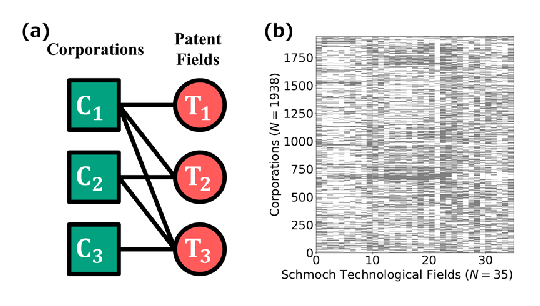
\includegraphics[scale=0.75]{Figs/Fig1.eps}
    \caption{(A) The legend of the five classifications defined by Schmoch \cite{Schmoch2008}, along with an explanation of the technology codes used in (B), (C), and (D).
    (B) Pearson correlation between \(k_{T,0}\) and \(k_{T,1}\) (\(r=0.064\)).
    (C) Pearson correlation between \(k_{T,0}\) and TCI (\(r=0.594\)).
    (D) Pearson correlation between TCI and \(k_{T,1}\) (\(r=0.316\)).
    In (B) through (D), the black lines indicate the mean values of \(k_{T,0}\) and \(k_{T,1}\), and \(\text{TCI} = 0\) is also shown with a black line. Each dot is color‐coded according to (A). The TCI values are unscaled.
    }
    \label{fig:scatter}
\end{figure}

\subsection*{Stability and Finer technological trends}

Traditional regional approach measures complexity as a relative index that reflects the outcomes of agglomeration economies at the country or city level \cite{hartmann2024economic} and relates to spatial inequality. 
This measure is strongly affected by the degree of urbanization in Japan. 
However, the regional approach depends on the aggregation level of regions or technologies \cite{Hidalgo2021}. 
When the HH algorithm is applied to patent data, finer classifications such as IPC classes lead to unstable behaviour of the complexity index when compared with coarse classifications such as the Schmoch system \cite{PintarEssletzbichler2022}. 
This instability applies to the evaluation of regional complexity and also occur in the evaluation of technology complexity owing to the symmetry of the bipartite network.

In this study we compare the TCI from the regional approach with the TCI from the corporate approach. We examine the differences in inequality and instability of complexity between regions and corporations by comparing results obtained with coarse and fine classifications (Panel A in Fig.~\ref{fig:detailtci}).

The scaled TCI of the Schmoch system shows that in the regional approach 26 out of 35 classes fall in the range of 75 to 100. 
In the corporate approach, only 15 classes lie in that range, whereas the other classes display greater differences among technologies in the regional approach. 
This difference in heterogeneity stems from the corporate approach being able to characterize each technology in a more detailed manner. The HH algorithm defines ubiquity as the degree of a technology node and this measure depends on the number of paired nodes. The regional approach has region nodes numbering in the tens up to fewer than 300 (for example the 47 prefectures). The corporate approach has corporation nodes numbering from one thousand to several ten thousand. The iterative calculation of TCI can therefore reflect a wider range of ubiquity.

The difference between the approaches also appears when using a finer classification. When the classification becomes more detailed and the number of technology nodes increases, the regional approach cannot define ubiquity sufficiently. In the case of Civil engineering the variance of TCI values for IPC classes corresponding to the same Schmoch class is larger than that for the corporate approach. The larger difference between the TCI values of the coarse classification and those of the finer classification indicates a greater instability in the evaluation for the regional approach. A Wilcoxon signed rank test shows that the distribution of residuals between the TCI values of the Schmoch and IPC classes is significantly different (p value = 7.225e-14) and that the residuals for the corporate approach are smaller than those for the regional approach (Panel B in Fig.~\ref{fig:detailtci}).

These stable and detailed trends are observed not only over a 30 year period but also in evaluations over shorter periods such as 5 years. For example, in the IPC classes corresponding to Food chemistry, the trend of high TCI is stable in the 2000s. Technologies with high scores (for example C13 and A21) and those that decline (for example A23 and A01) are captured in a consistent manner (SI Fig.~\ref{fig:bump}).

The corporate approach also permits a relative evaluation of technologies in a specific region that was not possible with the regional approach. The regional approach evaluates each region only by whether it possesses a technology that has been relatively evaluated at the national level. The corporate approach can assess which technology is important within that region. For example, the relationship between the TCI of each IPC class for three prefectures with many corporations and the TCI for all corporations shows that Aichi, the prefecture where a lot of co-manufacturing companies, such as Toyota, exhibits a trend different from Tokyo and Osaka (Fig.~\ref{fig:prefcompare}). In Aichi, the technologies with a relatively high evaluation even though the overall evaluation is low are the strengths of corporations located in that region.


\begin{figure}[ht]
    \centering
    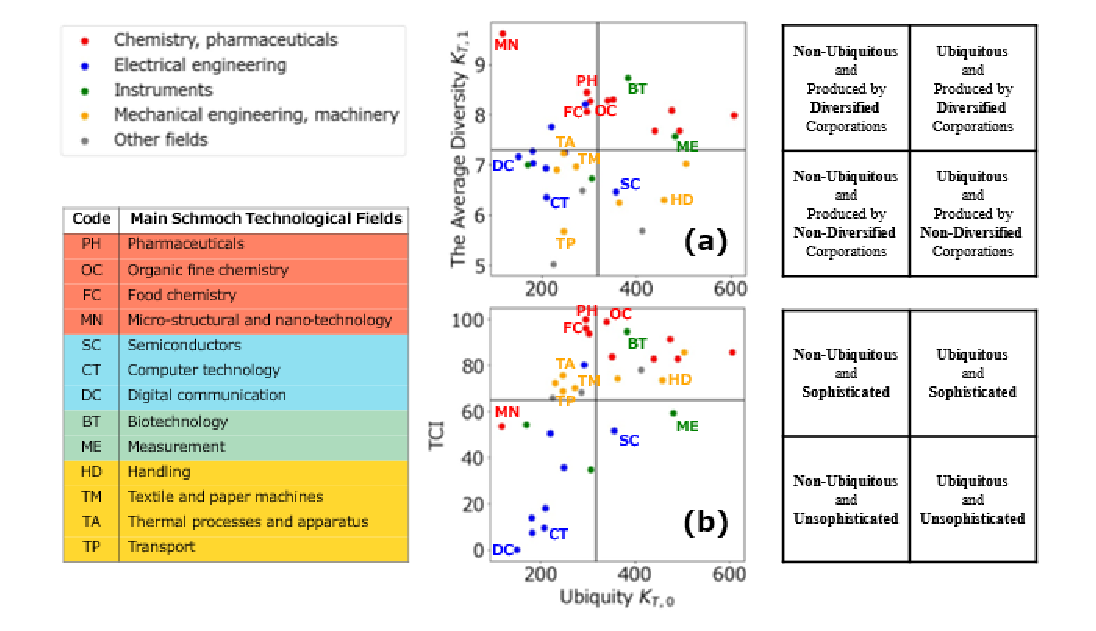
\includegraphics[scale=0.65]{Figs/Fig2.eps}
    \caption{(A) The TCI scores of IPC first Class (N=124) and Schmoch (N=35) for both prefectures and corporations. The scores have been scaled to values ranging from 0 to 100. Each IPC is plotted against the corresponding Schmoch axis, and in cases of many-to-many correspondences, each pair is plotted individually. (B) The distribution of the absolute differences between TCI of IPC and of Schmoch systems.}
    \label{fig:detailtci}
\end{figure}


\begin{figure}[ht]
    \centering
    \includegraphics[scale=0.35]{Figs/Fig3.eps}
    \caption{Three scatter plots arranged in a single row compare the Corporate TCI in Japan (vertical axis) to the Corporate TCI in Tokyo (left panel), Osaka (middle panel), and Aichi (right panel) on the horizontal axis. Each axis is scaled from 0 to 100, and the black points represent data points for each classification or entity. The red dashed line indicates the diagonal (y = x).}
    \label{fig:prefcompare}
\end{figure}

\section*{Discussion} \label{section:Discussion}
% The Discussion should be succinct and must not contain subheadings.

In this study, we applied TCI for the first time in Japan, targeting corporations and all patent technology fields, to identify sophisticated technological areas that are key to fostering innovation. Our findings highlighted high complexity in the pharmaceuticals and chemistry sectors, which may reflect the societal conditions of the period, often referred to as the dawn of the pharmaceutical industry in Japan. This era was marked by significant technological advancements and innovation in these fields.
While it has been argued that the evaluation results of these technological fields may converge due to their classification methods \cite{Hidalgo2021}, the corporate-level approach achieved stable evaluations even when using fine classifications. This contrasts with the traditional regional approach, which often relies on coarse classifications to maintain stability. The ability of the corporate approach to deliver consistent results at a finer granularity suggests its potential to provide more accurate and detailed insights into technological trends within specific regions, industries, or other limited scopes.
Despite the above findings and the advances, there remain areas where the corporate approach must demonstrate its robustness and usefulness in ways that the traditional regional method has successfully addressed. 
First, capturing changes in technological trends effectively requires not only long-term analyses but also short-term evaluations, which are essential for identifying emerging fields and shifts in innovation patterns. However, such analyses introduce challenges in data processing. For instance, the calculation of the TCI is sensitive to the number of patents by corporation and technological field in each period. Shortening the aggregation period may lead to the inclusion of corporations with a minimal number of patents, potentially introducing noise into the TCI calculations and affecting the stability of results \cite{PintarEssletzbichler2022}.
This issue stems from a limitation in the HH algorithm, which evaluates network complexity based on node degrees in a bipartite graph. The reliance on node degrees relaxes the conditions for link formation, particularly when dealing with sparse data. To address this limitation, several mathematical and algorithmic improvements have been proposed. For example, the Fitness--Complexity (FC) algorithm by Tacchella et al. \cite{Tacchella2012} incorporates non-linear iterative calculations to better account for the structure of the network. This algorithm has demonstrated strong correlations with HH--based indicators while offering improved robustness in evaluating regional and corporate competitiveness \cite{Wu2016,Albeaik2017}.
By integrating such enhancements into this approach, the analysis could derive deeper insights into Japan's industrial technology landscape. 
Future work should explore not only the application of these improved methods but also comparisons of the insights obtained through the corporate approach with results from other countries. Such comparative analyses would help elucidate the distinctive characteristics of Japanese corporations in the context of intensifying global competition.

Second, the ad-hoc nature of certain data processing steps detailed in Data\ref{subsection:Data} section, such as the exclusion of corporations with few patents, highlights the need for more systematic and scalable solutions. Addressing these issues through algorithmic refinements rather than manual interventions could enhance the accuracy and reliability of the results.

Ultimately, this study represents a cornerstone for understanding the characteristics of domestic industries in Japan through the lens of technological complexity. By identifying key technological areas, the findings offer valuable insights that can inform industrial policies and strategies, especially in an era marked by rapid advancements in artificial intelligence and increasing international competition.


\section*{Methods} \label{section:Methods}
\subsection*{Data} \label{subsection:Data}
The dataset used in this study consists of registered patents applied to the Japan Patent Office (JPO) over a 30-year period from fiscal 1981 to 2010. The data comprises detailed records of 3,189,536 patents filed by 64,622 corporations. Patent records follow the International Patent Classification (IPC) system and are further organized according to the Schmoch classification \cite{Schmoch2008}. 

The Schmoch system aggregates IPC codes into 35 distinct technological fields, ensuring balanced class sizes and technological consistency. The Schmoch grouping has received widespread application in previous studies \cite{PintarScherngell2022,Balland2018,Whittle2019}.
Regarding how to utilize a patent to measure contribution, traditional approaches have relied on raw patent counts to measure technological contributions in various fields \cite{Balland2016,Balland2018,PintarScherngell2022,Pinheiro2022,Whittle2019,Jun2023,Abay2024}. However, as highlighted by Pintar et al.\ \cite{PintarScherngell2022}, simple counts may overestimate contributions when a patent involves multiple corporations or spans several technological fields.
To address this issue, the primary IPC class of each patent is mapped onto the corresponding Schmoch field, and the value of a patent is fractionally allocated by dividing it equally among all associated corporations and among all technological fields to which it is attributed. This procedure prevents overestimation of contributions from a corporation or a field due to multiple co-ownership or cross-field classification.
Although the raw dataset spans a wide range of patenting activity, most corporations show only minimal engagement such as holding a single patent in one field (SI Fig. \ref{fig:patentdistribution}). 
Low-activity cases may distort link formation in network analyses based on the HH algorithm \cite{PintarScherngell2022}. 
For this reason, a filtering criterion based on the distribution of patent counts per corporation is therefore applied, retaining only the top 3\% in terms of patent output. After filtering, the dataset consists of 2,485,027 patents from 1,938 corporations, representing approximately 93\% of the original patent count.

In order to quantify specialization in technological fields, computation of the revealed technological advantage (RTA)\cite{Soete1987} index which builds on the revealed comparative advantage framework\cite{Balassa1965} is necessary.
The RTA index for a given corporation in a specific technological field measures the ratio between the share of patents held by corporation \(C\) in technology \(T\) and the share of patents in technology \(T\) among all corporations.
Let \(W_{C,T}\) denote the weighted patent count for corporation \(C\) in technology \(T\), where each patent is assigned a weight computed as one divided by the product of the number of associated corporations and the number of technological classes assigned to the patent.
The numerator of the RTA index captures the fraction of patent activity devoted to technology \(T\) for corporation \(C\). 
Similarly, the denominator reflects the overall share of patent activity in technology \(T\) among all corporations, computed as the sum of \(W_{CT}\) over all corporations divided by the sum of \(W_{CT}\) over all corporations and technologies.
The RTA index is thus given by

\begin{center} \label{eq1}
    \begin{equation}
    \mbox{RTA}_{CT} = \frac{W_{CT}}{\sum_{T} W_{CT}} \Bigg/ \frac{\sum_{C} W_{CT}}{\sum_{CT} W_{CT}}~.
    \end{equation}
\end{center}
We consider that RTA index values of 1 or greater indicate that corporation \(C\) holds a prominent technological advantage in technology \(T\). Based on this threshold, a binary adjacency matrix of the bipartite network \(M_{CT}\) is defined by

\begin{center}
\begin{equation} \label{eq2}
M_{CT} = 
\begin{cases} 
1 & \text{if } \mbox{RTA}_{CT} \geq 1, \\
0 & \text{otherwise}.
\end{cases}
\end{equation}
\end{center}


\subsection*{Technological Complexity} \label{TCI}
The binary matrix \(M_{CT}\) forms the two metrics which characterize each node in the bipartite network by the sum of connections, known as degree centrality. The diversity of corporations \(K_{C,0}\) quantifies the number of technologies in which a corporation is specialized, and indicated by $M_{CT}$. 
Similarly, the ubiquity of technologies \(K_{T,0}\) represents the number of corporations that exhibit a technological advantage in a given field. These quantities are computed as

\begin{equation}\label{eq3}
\begin{aligned}
K_{C,0} = \sum_{T} M_{CT},  
K_{T,0} = \sum_{C} M_{CT}~.
\end{aligned}
\end{equation}

Higher diversity values indicate corporations with broad technological capabilities, while lower ubiquity values signify that the technologies are rare. 
Through calculating these two characteristics of adjacent nodes iteratively, the diversity and ubiquity of each node is updated as

\begin{equation}\label{eq4}
K_{C,N} = \frac{1}{K_{C,0}} \sum_{T} M_{CT}\, K_{T,N-1},
\end{equation}

\begin{equation} \label{eq5}
K_{T,N} = \frac{1}{K_{T,0}} \sum_{C} M_{CT}\, K_{C,N-1}.
\end{equation}

Here, the metric \(K_{T,1}\) represents the average nearest neighbor degree for technology nodes and it reflects the average diversity of corporations connected to a given technology.
Substituting Eq. \ref{eq4} into Eq. \ref{eq5} yields

\begin{equation} \label{eq6}
K_{T,N} = \sum_{T'} \widetilde{M}_{TT'} K_{T',N-2}
\end{equation}

where \(T'\) denotes a technological field, and $\widetilde{M}_{TT'}$ is defined as

\begin{equation} \label{eq7}
\widetilde{M}_{TT'} = \sum_{C} \frac{M_{CT}\, M_{CT'}}{K_{C,0}\, K_{T,0}}~.
\end{equation}

Eq. \ref{eq6} is satisfied when  \(K_{T,N} = K_{T,N-2} = 1\), which corresponds to the eigenvector associated with the largest eigenvalue of the stochastic matrix \(\widetilde{M}_{T,T'}\). 
Since this eigenvector is a vector of ones and not informative, the eigenvector corresponding to the second largest eigenvalue of \(\widetilde{M}_{TT'}\) captures the greatest variance among technology fields \cite{Hidalgo2021, Mealy2019}.
Thus, TCI is given by
\begin{equation} \label{eq8}
TCI = \frac{\widetilde{T} - \langle \widetilde{T} \rangle}{\text{stdev}(\widetilde{T})},
\end{equation}

where \(\widetilde{T}\) represents the eigenvector corresponding to the second largest eigenvalue of \(\widetilde{M}_{TT'}\), and \(\langle \widetilde{T} \rangle\) is their mean and \(\text{stdev}(\widetilde{T})\) is their standard deviation.



\bibliography{ref}

% \noindent LaTeX formats citations and references automatically using the bibliography records in your .bib file, which you can edit via the project menu. Use the cite command for an inline citation, e.g.  \cite{Hao:gidmaps:2014}.

% For data citations of datasets uploaded to e.g. \emph{figshare}, please use the \verb|howpublished| option in the bib entry to specify the platform and the link, as in the \verb|Hao:gidmaps:2014| example in the sample bibliography file.

% \section*{Acknowledgements (not compulsory)}
% Acknowledgements should be brief, and should not include thanks to anonymous referees and editors, or effusive comments. Grant or contribution numbers may be acknowledged.

\section*{Author contributions}
H.I. collected the data and secured the funding. R.K. designed the study, conceived the main research idea, performed the analysis, and drafted the manuscript. Both H.I. and R.K. critically reviewed the results, contributed to the revisions of the manuscript, discussed the findings, and approved the final version of the manuscript.

% Must include all authors, identified by initials, for example:
% A.A. conceived the experiment(s),  A.A. and B.A. conducted the experiment(s), C.A. and D.A. analysed the results.  All authors reviewed the manuscript. 

\section*{Additional information}

To include, in this order: \textbf{Accession codes} (where applicable); \textbf{Competing interests} (mandatory statement). 

The corresponding author is responsible for submitting a \href{http://www.nature.com/srep/policies/index.html#competing}{competing interests statement} on behalf of all authors of the paper. This statement must be included in the submitted article file.
% \begin{figure}[ht]
%     \centering
%     \includegraphics[scale=0.5]{Figs/FigA.eps}
%     \caption{The bibpartite network of corporations and technological fields. The edges represent that the corporations produce technologies in the fields.}
%     \label{fig:bipartite}
% \end{figure}
\renewcommand{\thefigure}{S\arabic{figure}}
\setcounter{figure}{0}

\begin{figure}[ht]
    \centering
    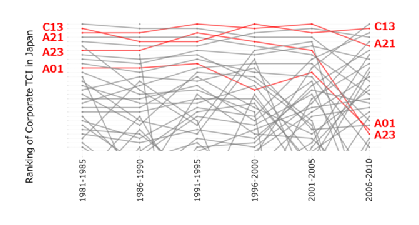
\includegraphics[scale=0.75]{Figs/FigA2.eps}
    \caption{The Pearson correlation between the degree centrality \( k_{T,0} \) of technology node \( T \) classified by IPC and the average nearest neighbor degree \( k_{T,1} \), and the Pearson correlation between the degree centrality \( k_{T,0} \) of technology field node \( T \) and TCI, scaled from 0 to 100. In both figures, the black lines indicate the mean values. Each data point is color-coded according to the five classifications defined by Schmoch\cite{Schmoch2008}.
    All figures were created using Python 3.10 and the matplotlib (3.4.3) package (https://matplotlib.org).}
    \label{fig:persector}
\end{figure}

\begin{figure}[ht]
    \centering
    \includegraphics[scale=0.85]{Figs/FigA3.eps}
    \caption{The top 30 TCI rankings in five year increments from 1981 to 2010. IPC classes associated with Food Chemistry (C13, A21, A23, and A01) are highlighted in red.
    All figures were created using Python 3.10 and the matplotlib (3.4.3) package (https://matplotlib.org).}
    \label{fig:bump}
\end{figure}

\begin{figure}[ht]
    \centering
    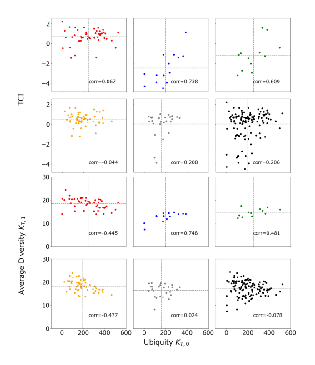
\includegraphics[scale=0.75]{Figs/FigA1.eps}
    \caption{The distribution of weighted patent counts (horizontal axis) for each corporation, with the cumulative distribution function (CDF) of their patents on the vertical axis. The black dashed lines on both axes indicate the excluded region, corresponding to the top 3\% of corporations that account for 93% of all patents.
    The figure was created using Python 3.10 and the matplotlib (3.4.3) package (https://matplotlib.org).}
    \label{fig:patentdistribution}
\end{figure}


\end{document}